%%%%%% This section should describe the signature or the methods you are trying to take advantage of %%%%%%
\section{Theory}
Alpha particles pose a problematic background in large granular detector arrays, particularly those that originate from Rn progeny that plate out on the detector surfaces during manufacturing and assembly. The \ppc\ detector technologies implemented in the \MJ\ \DEM\ have a thick (1-2 mm) outer dead layer covering most of the detector surface that is insensitive to alpha interactions originating external to or on the surface of the detector, and the point contact, despite being sensitive to these alphas, is very small in size. These features make HPGe detector arrays inherently less sensitive to alphas than, for example, bolometric arrays. 

However, between the point contact and the outer dead layer is a thin passivated surface; its response to alphas is less easy to characterize. The charge collection properties near this surface can differ for different detector models. In the \textsc{Majorana Demonstrator}, events have been observed in which alphas originating on this surface are significantly degraded in energy, leading to a potential background contribution in the region-of-interest for neutrinoless double-beta decay. 

However, it is also observed that charge mobility is drastically reduced on or near the passivated surface, and is slowly released on the timescale of waveform digitization, leading to a measurable decrease in the slope of the tail of a recorded pulse. The same effect has been observed in the TUBE alpha source scans (see unidoc).

There are two models for charge loss in the passivated surface region. One option is that this effect is due to surface propagation of the electron contribution to the signal, with the holes being collected normally. This matches the model developed in \cite{Mullowney2012}. See Fig.~\ref{fig:siggen_wf} for sample waveforms, simulated using siggen. 

\begin{figure}[h]
 \centering
 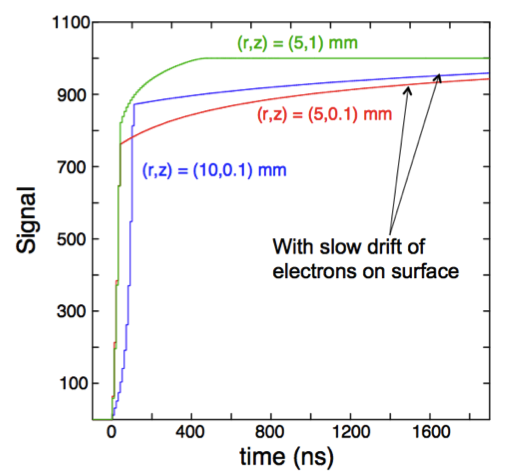
\includegraphics[height=3in]{/Users/jgruszko/Documents/Thesis/Plots/Ch3/siggen_wf}
 \caption[Simulated bulk and passivated surface waveforms]{Bulk and passivated-surface waveforms, simulated using siggen. Surface charge transport of electrons is induced by incorporating an arbitrary small amount of passivated-surface charges in the fieldgen model of the detector, which leads to electric field lines that end on the passivated surface.} 
 \label{fig:siggen_wf}
\end{figure}

In an alternative model, holes are trapped when they originate in a few-micron-thick region at the passivated surface, and then slowly re-released. Since the alpha particle's path in the detector carries it through this region and into the normal-collection bulk region, part of the energy of the event appears as a normal, fast pulse, and the remainder of the charge is collected slowly. The waveforms of the events would appear similar to those including surface electron transport. The bulk trapping and slow surface drift effects could also appear in conjunction. 

The models behave differently as the position of the alpha interaction on the passivated surface changes, so they can be distinguished using the TUBE scan results (see Sec.~\ref{sec:dcr_models}). For the purposes of this analysis, the cause of the delayed charge is irrelevant. 

Using a filter that can identify the occurrence of this delayed charge recovery, these events can be identified, allowing for the efficient rejection of passivated surface alpha events in analysis. The goal of such a filter is to detect the presence of slow charge collection occurring after the bulk charge collection has been completed. In a waveform that has been fully corrected for the electronic response function, this appears as a positive slope of the tail. In an uncorrected pulse, it appears as a tail which has a less-negative slope than is expected for that particular channel's electronics response. 

%%%%%% In this section you should validate your techniques. %%%%%% 
\section{Implementation}
For all versions of the DCR analysis cut, the relevant parameters are found using calibration data, since these runs contain a very low fraction of surface events. Version 1.0 is the version of the analysis currently in use in the \MJ\ \DEM\ analysis chain, and does not require knowledge of the electronics response function. Version 1.1 is identical to version 1.0, but with an added term that corrects for charge trapping in the bulk of the detector, reducing systematic uncertainties. It is currently under development. Version 2.0 is a proposal to be implemented in future analysis of \MJ\ \DEM\ data, which uses a full correction for the electronics response function. Optimization and error estimates are fully described for version 1.0 of the analysis, and commented on in a more limited capacity for the other versions. 

\subsection{DCR Version 1.0}
The DCR parameter is found by first calculating the slope of the waveform tail for each event in a channel. 1 $\mu$s of the waveform is averaged (corresponding to 100 waveform samples in non-multisampled data) at each of two points on the waveform. The first region lies between 2 and 3 $\mu s$ after 97\% of the waveform rise, and the second is the final $\mu s$ of the waveform (in the non-multisampled data, this is between 19 and 20 $\mu s$). See Fig.~\ref{fig:DCR_step1}. These values were chosen to avoid introducing unwanted sensitivity to the shape of the waveform turnover and to decrease sensitivity to noise. Waveforms for which no valid tail slope can be found, i.e. those in which the 97\% time point occurs too late to leave a usable tail, are flagged and automatically accepted by the DCR analysis. 

\begin{figure}[h]
 \centering
 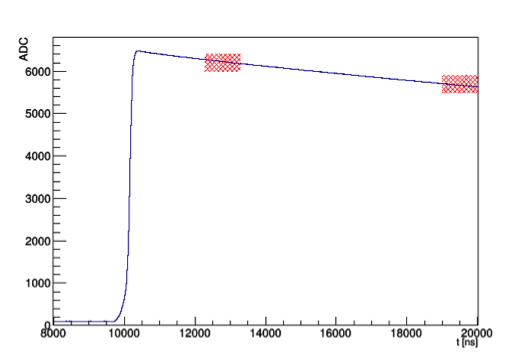
\includegraphics[height=2in]{/Users/jgruszko/Documents/Thesis/Plots/Ch3/DCR_step1}
 \caption[A sample MJD waveform, with indicated tail slope measurement points]{A sample MJD waveform. The ADC values are averaged in each of the two shaded regions. The slope between those average points is taken to be $\delta$.} 
 \label{fig:DCR_step1}
\end{figure}

\begin{figure*}[t]
 \centering
 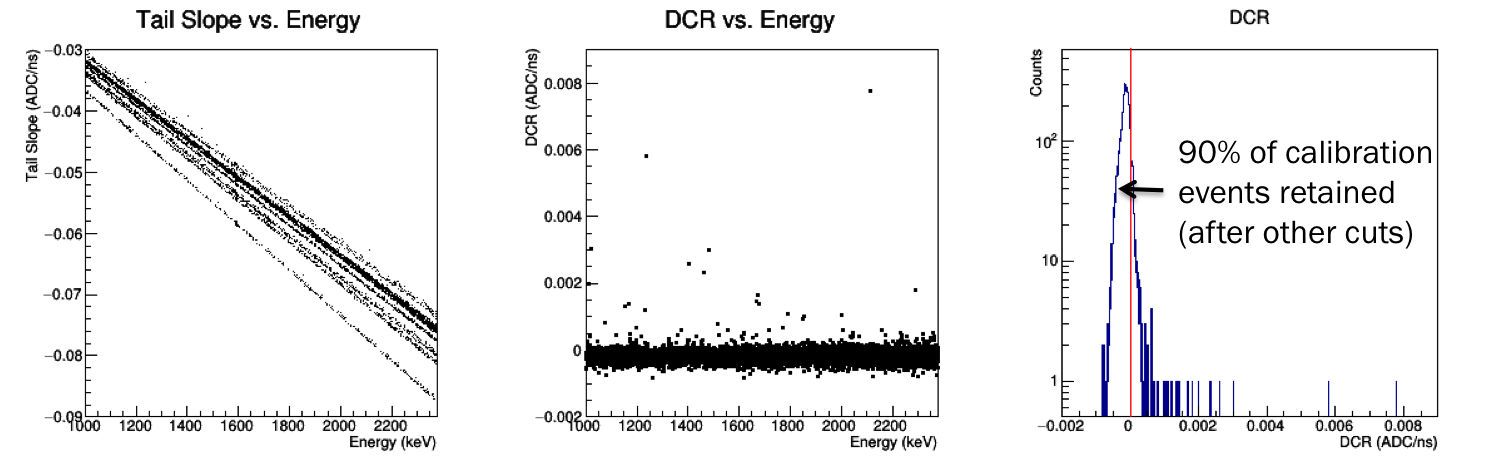
\includegraphics[width=1.0\textwidth]{/Users/jgruszko/Documents/Thesis/Plots/Ch3/DCR_implementation}
 \caption[The steps of the DCR parameter calculation]{The steps of the DCR parameter calculation, plotted for all high gain channels in DS3 detectors. {\it Left:} $\delta$ vs. Energy is plotted and fit with a line for each channel. {\it Center:} The fit parameters are used to calculate the raw DCR value, which is then shifted such that 90\% of single-site calibration events in this energy range fall below 0. {\it Right:} The DCR distribution displays a gaussian distribution with a high-DCR tail.} 
 \label{fig:DCR_implementation}
\end{figure*}

Assuming that the tail of bulk-event waveforms has an exponential form, the slope $\delta$ is:
$$\delta = \frac{y_1 - y_2}{t_1-t_2} = A\frac{e^{\frac{-t_1}{\tau}}-e^{\frac{-t_2}{\tau}}}{t_1-t_2} $$
where $y_1$, $y_2$, $t_1$ and $t_2$ correspond to the average values and times for each of the two regions, $A$ is the waveform amplitude, and $\tau$ is the decay constant of the tail. 

To first order in $t_n/\tau$, 
$$\delta = \frac{A}{\tau}$$
for bulk events. 

The tail slope is plotted with respect to energy for each channel. Using single-site events with energies between 1\,MeV and 2.38\,MeV (the Compton shoulder of the $^{208}$Th 2614 keV peak), a line is fit to the resulting distribution, and the parameters of that fit are used to project $\delta$ on to the energy axis. This is equivalent to finding the average decay constant for the pulses in a channel and doing a first-order pole-zero correction of the waveforms prior to measuring their tail slope. 

The resulting value is defined as the raw DCR parameter for the waveform:
$$\mathit{DCR_{raw}} = \Delta - (\frac{a}{\tau}E+b)$$
where $a$ is a scaling constant that converts between pulse amplitude and energy for the channel. $b$, which is generally positive, is a constant determined by the fit that corrects for the fact that a waveform with signal height 0 will have a positive estimated energy when the maximum value of a trapezoidal filter is used as the energy estimate. 

The calibration run events have a median raw DCR of 0, with low tail slope events (i.e. events occurring near the passivated surface) having larger DCR values. The width of the gaussian part of the DCR distribution in the calibration data is primarily determined by the noise and energy nonlinearity of the channel. The high-DCR tail is due to passivated-surface events, transition-layer multisite events (see Fig.~\ref{fig:DCR_PS}) and other multi-site events that go untagged by A/E and pile-up cuts, and an additional contribution that depends on the bulk charge trapping of the detector (see Sec.~\ref{ssec:dcr_ct} for details). 

The cut value $c$ is set to reject 1\% of the single-site events with energies between 1\,MeV and 2.38\,MeV in the calibration data set used to determine the cut parameters. Single-site events are selected using  A vs. E analysis and additional pile-up cleaning cuts (see Data Cleaning unidoc section).
To set the ``corrected DCR" (DCR\textsubscript{corr}) value (hereafter referred to simply as ``DCR"), the raw DCR value is shifted such that the rejected events have DCR\textsubscript{corr}$>0$:
$$\mathrm{DCR}\textsubscript{corr} = \Delta - (\frac{a}{\tau}E+b) - c$$
This value is then calculated for all background events. 


\subsection{Energy Non-Linearity Effect}
The non-linearity of the waveform digitization has a significant effect on the efficiency of the cut at a given energy. Though much of the variation in efficiency is removed by nonlinearity correcting each waveform \cite{EnergyUnidoc}, a systematic variation with energy remains, as seen in the variation of the Compton continuum acceptance in  Figure \ref{fig:dcr99_eff}. This effect differs from channel to channel, with low-gain channels displaying higher variation. The variation due to this effect is highly dependent on the chosen bulk acceptance efficiency; at high acceptance levels, the effect is greatly reduced. 

\begin{figure}[t]
 \centering
 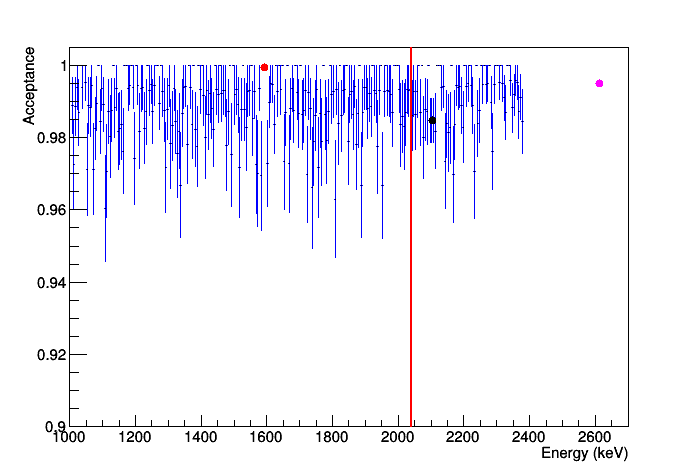
\includegraphics[height = 3in]{/Users/jgruszko/Documents/Thesis/Plots/Ch3/Ch640_dcr99_eff.png}
 \caption[99\% acceptance DCR cut efficiency and uncertainties]{Efficiency plot for the 99\% acceptance DCR cut in P42665A, a typical detector in DS3. The acceptance in the $^{208}$Th DEP, SEP, and FEP are indicated by the red, black, and magenta points, respectively. The blue points indicate the acceptance in each 5\,keV bin of the Compton continuum. The red line indicates the 3\,keV \nonubb\ ROI.} 
 \label{fig:dcr99_eff}
\end{figure}

This cannot be correctly termed an uncertainty of the cut, since the energy of a given event is well-known, as is the DCR efficiency at a given energy. A gain uncertainty of 0.4\,keV, larger than that observed in any data set \cite{EnergyUnidoc} leads to a DCR efficiency change of less than 0.2\%, which is negligible compared to the other DCR uncertainties, so this uncertainty is neglected. 

The non-linearity effect will change the spectral shape of the remaining events, however. When estimating an integral rate over some region, the DCR acceptance should be calculated for that particular region, so that bias is not introduced. For the \nonubb\ limit calculation, the DCR efficiency is calculated in a 3\,$\sigma$-window around the \nonubb\ Q-value. 

\subsection{Optimization}
As described in \cite{Detwiler_sensitivity}, the sensitivity to the \nonubb\ decay half-life, in the presence of backgrounds, is proportional to $\frac{\epsilon}{\sqrt{N_b}}$, where $\epsilon$ is the cut acceptance and $N_b$ is the number of background events. In this case, the energy range used to find the number of background events is the disjoint 350\,keV window around the \nonubb\ Q-value that is used to estimate the background level in the ROI. The event energies included those from 1950 to 2350\,keV, with the exception of the regions from 2094 to 2127\,keV and 2195 to 2212\,keV, where the \MJ\ background model predicts the presence of gamma background peaks. 

An optimization study was conducted using the open data from \MJ\ \DEM\ data sets 0 to 4. See Table.~\ref{tab:DS_summary} for descriptions and exposures of each data set. Data set 5 was excluded from this study due to the known elevated noise rate in its first half, which distorts the DCR distribution and reduces the effectiveness of the analysis. Only enriched detectors were included in the optimization study, since these detectors dominate the \DEM 's sensitivity to \nonubb . 

For this study, the sensitivity was evaluated at a range of DCR calibration-event acceptance levels, varying from 90\% to 100\%. See Table~\ref{tab:DCR_opt}. Based on the results, the DCR acceptance level was chosen to be 99\%. 

Higher acceptance levels are being considered for multi-sampled data, since the longer duration of the waveform tail leads to a more-sharply peaked DCR distribution for bulk events. See Figure~\ref{fig:DS2_DS3_comparison}. Though the open exposure in this data set is low, and higher statistics are needed to make a definitive recommendation, studies of DS 2 suggest that a 99.9\% acceptance DCR cut may be the optimal choice for multi-sampled data. Acceptances over 99\% were also studied in DS 0-1 and 3-4 and were found to be suboptimal. 

\begin{table}[]
\centering
\begin{tabular}{l l | l l l l}
DS &  $\epsilon$ (\%) & $N_{b}$ (counts) & $\frac{N_{b}}{\epsilon}$ (arb.) & $N_{b, enr}$ (counts) &$\frac{N_{b, enr}}{\epsilon}$ (arb.) \\    
\hline
0 &                  100 &        79 &             1.13e-01$\pm$5.63e-02 &                   69 &             1.20e-01$\pm$6.02e-02 \\
 &                   99 &        14 &             2.65e-01$\pm$1.32e-01 &                   10 &             3.13e-01$\pm$1.57e-01 \\
 &                   95 &        14 &             2.54e-01$\pm$1.27e-01 &                   10 &             3.00e-01$\pm$1.50e-01 \\
 &                   90 &        14 &             2.41e-01$\pm$1.20e-01 &                   10 &             2.85e-01$\pm$1.42e-01 \\
\hline
1 &                  100 &      49 &             1.43e-01$\pm$7.14e-02 &                   46 &             1.47e-01$\pm$7.37e-02 \\
 &                   99 &       6 &             4.04e-02$\pm$2.02e-02 &                    3 &             5.72e-02$\pm$2.86e-02 \\
 &                   95 &       6 &             3.88e-02$\pm$1.94e-02 &                    3 &             5.48e-02$\pm$2.74e-02 \\
 &                   90 &       6 &             3.67e-02$\pm$1.84e-02 &                    3 &             5.20e-02$\pm$2.60e-02 \\
\hline               
2 &                  100 &      7 &             3.78e-01$\pm$1.89e-01 &                    6 &             4.08e-01$\pm$2.04e-01 \\
 &                   99.9 &       0 &                  inf$\pm$inf &                    0 &                  inf$\pm$inf \\
 &                   99.5 &       0 &                  inf$\pm$inf &                    0 &                  inf$\pm$inf \\
 &                   99 &       0 &                  inf$\pm$inf &                    0 &                  inf$\pm$inf \\
 &                   95 &       0 &                  inf$\pm$inf &                    0 &                  inf$\pm$inf \\
 &                   90 &       0 &                  inf$\pm$inf &                    0 &                  inf$\pm$inf \\
\hline              
3 &                  100 &     25 &             2.00e-01$\pm$1.00e-01 &                   21 &            2.18e-01$\pm$1.09e-01 \\
 &                   99 &      2 &             7.00e-01$\pm$3.50e-01 &                    0 &                  inf$\pm$inf \\
 &                   95 &      2 &             6.72e-01$\pm$3.36e-01 &                    0 &                  inf$\pm$inf \\
 &                   90 &      2 &             6.36e-01$\pm$3.18e-01 &                    0 &                  inf$\pm$inf \\
\hline
4 &                  100 &     17 &             2.43e-01$\pm$1.21e-01 &                   16 &             2.50e-01$\pm$1.25e-01 \\
 &                   99 &      1 &             9.90e-01$\pm$4.95e-01 &                    0 &                  inf$\pm$inf \\
 &                   95 &      1 &             9.50e-01$\pm$4.75e-01 &                    0 &                  inf$\pm$inf \\
 &                   90 &      1 &             9.00e-01$\pm$4.50e-01 &                    0 &                  inf$\pm$inf \\
\end{tabular}
 \caption[DCR optimization studies for the \DEM ]{DCR optimization studies in DS 0 to 4 show that the sensitivity of the cut is optimized at 99\%. Results in DS2 suggest that higher acceptances, up to 99.9\%, may be optimal when multi-sampling is used.} 
 \label{tab:DCR_opt}
\end{table}


\begin{figure}[h]
 \centering
 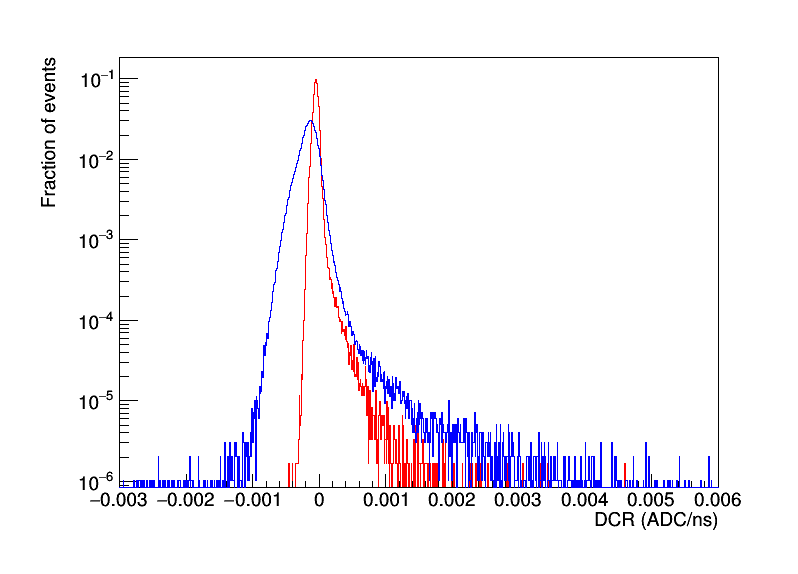
\includegraphics[height=3in]{/Users/jgruszko/Documents/Thesis/Plots/Ch3/DS2_DS3_cont_forUnidoc.png}
 \caption[Comparison of DCR in singly-sampled and multi-sampled MJD data sets]{DCR of single-site Compton continuum events in calibration data, in multisampled data (DS2, in red) and singly-sampled data (DS3, in blue). In DS 2, DCR is more sharply peaked for bulk events, allowing for a higher-acceptance DCR cut that retains the same sensitivity to alpha events.} 
 \label{fig:DS2_DS3_comparison}
\end{figure}


\subsection{Uncertainty Estimation}
\subsubsection{Stability}
To study DCR stability over time, calibration skim files are chained together and analyzed.  DCR values for every event are plotted as a function of time, with time presented as the number of minutes elapsed since the beginning of the first calibration, with non-calibration periods removed from the timeline. See Fig.~\ref{fig:DS3_stab}, {\it top}. Only calibrations from the Module 1 source are used in the DS0-DS3 analysis, and only calibrations from the Module 2 source are used in the DS4 analysis.  Calibrations from both sources are used in the DS5 analysis. Calibration runs with timing or quality issues are removed from all analyses.  

Only single-site (as determined by {\tt avse} and {\tt nX} cuts) events in ``{\tt isGood}" detectors that pass data-cleaning cuts are included in the analysis. The energy window used for the \nonubb\ analysis is 2028\,keV - 2050\,keV. A second analysis of the $^{208}$Tl DEP (1590\,keV - 1595\,keV) is also conducted. A 40-minute moving average of the DCR values within the closed range [-0.003,0.035] is calculated. The larger upper bound was chosen to catch events with a high DCR due to mis-calibrations in the energy parameter {\tt trapENMCal}. The mean DCR value is then plotted at the central time value within each forty-minute window (see Fig.~\ref{fig:DS3_stab}, {\it middle}). Data points from the first and last forty minutes are excluded to eliminate bias due to window effects. 

The DCR cut efficiency (i.e.  the percentage of events within the window with {\tt dcr90<0}) over time is plotted using the same moving-average algorithm, as in Fig.~\ref{fig:DS3_stab}, {\it bottom}. Note that this method of calculating efficiency differs from the standard efficiency calculation, which weights each detector's efficiency by its active mass.  An effort to employ this method in the stability analysis is currently under development. A one-dimensional histogram is created out of the efficiency values over time, and the standard deviation of this distribution is taken to be the uncertainty in the efficiency of DCR over time, $\sigma_{stab}$. 

This analysis is conducted for high- and low-gain channels in each data set. Results are given in Table~\ref{tab:DS_efficiencies}. If the efficiency deviates by more than $2\sigma_{stab}$ in a set of calibration runs, the DCR parameters are re-evaluated using the relevant runs and a stability correction is applied. Stability corrections to DCR are also applied when a stability correction is needed in the A vs. E analysis \cite{AvsE_unidoc}.

The current version of the analysis employs one to two longer (8 to 12 hour) energy calibrations to set the cut in each data set. 

\begin{sidewaysfigure}[]
 \centering
 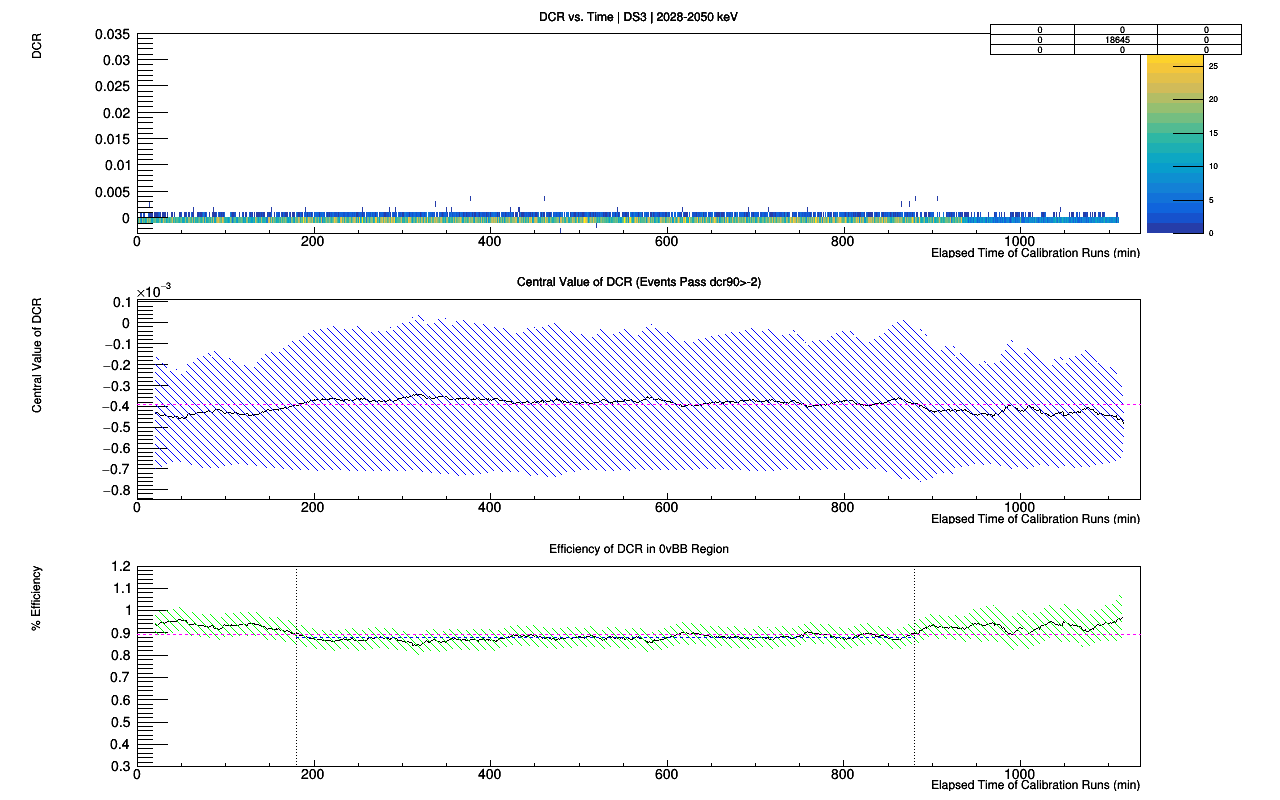
\includegraphics[width=1.0\textwidth]{/Users/jgruszko/Documents/Thesis/Plots/Ch3/DS3_stab}
 \caption[DCR stability study results in DS3 high-gain channels]{Stability study results for DS3 high-gain channels. The middle and bottom figures are calculated using a 40-minute moving average; in these plots the filled dashed region indicates the uncertainty in each value, taken as the standard deviation of the value's distribution in a given time window. The magenta lines indicate the mean of the plotted values. {\it Top:} DCR values for all events passing cuts. {\it Middle:} The central value of DCR over time. {\it Bottom:} The bulk acceptance of the DCR cut over time. The vertical lines indicate the runtime boundaries of the long calibration run used to set the DCR cut, and the blue line indicates the average efficiency in this time window. Plots courtesy of Chris Haufe.} 
 \label{fig:DS3_stab}
\end{sidewaysfigure}


\subsubsection{Statistical Uncertainty}
In each channel, the statistical uncertainty of the cut efficiency is $\frac{\sigma}{N} = \frac{1}{\sqrt{N}}$, where $N$ is the number of events rejected by the DCR cut in the set of calibration runs used to set the cut, in the energy window being used. See Table~\ref{tab:DS_efficiencies} for the uncertainties in the \nonubb\ efficiency window.

\subsubsection{Pulse-Shape Bias}
Irregularities in the pulse shapes of events, particularly charge-trapping re-release and multi-site effects, can have an effect on the calculated DCR acceptance. Events with a transition layer multi-site component, multi-site events occurring very near the point contact, and events with high charge trapping, like those seen in \ref{fig:DCR_PS}, may be untagged by A vs. E and data cleaning analyses, but will be accepted by the DCR cut with lower-than-average efficiency. A visual examination of the calibration events rejected based on their DCR values shows many of them to be of this type.

To quantify the uncertainty introduced by these effects, we compare the DCR acceptance in a 3$\sigma$ window centered on the $^{228}$Th double-escape peak (DEP), a known sample of single-site events, to the average acceptance in the left- and right-hand sidebands of the peak. The difference is cited as the pulse shape-dependent bias ($\sigma_{PS}$) for each channel. This value is generally positive, indicating that the acceptance in the DEP is higher than the average acceptance, and therefore that we have taken a conservative estimate of the DCR efficiency. The overall bias is given by an exposure-weighted average of the bias in each channel, since $\sigma_{PS}$ is assumed (conservatively) to be fully correlated among the detectors. 

The pulse shape bias indicates that the DCR analysis is effectively tagging some fraction of the multisite gamma events that go untagged by the A vs. E analysis. This implies that the DCR analysis has power for rejecting background gamma events in addition to alpha events.

\begin{figure}[]
 \centering
 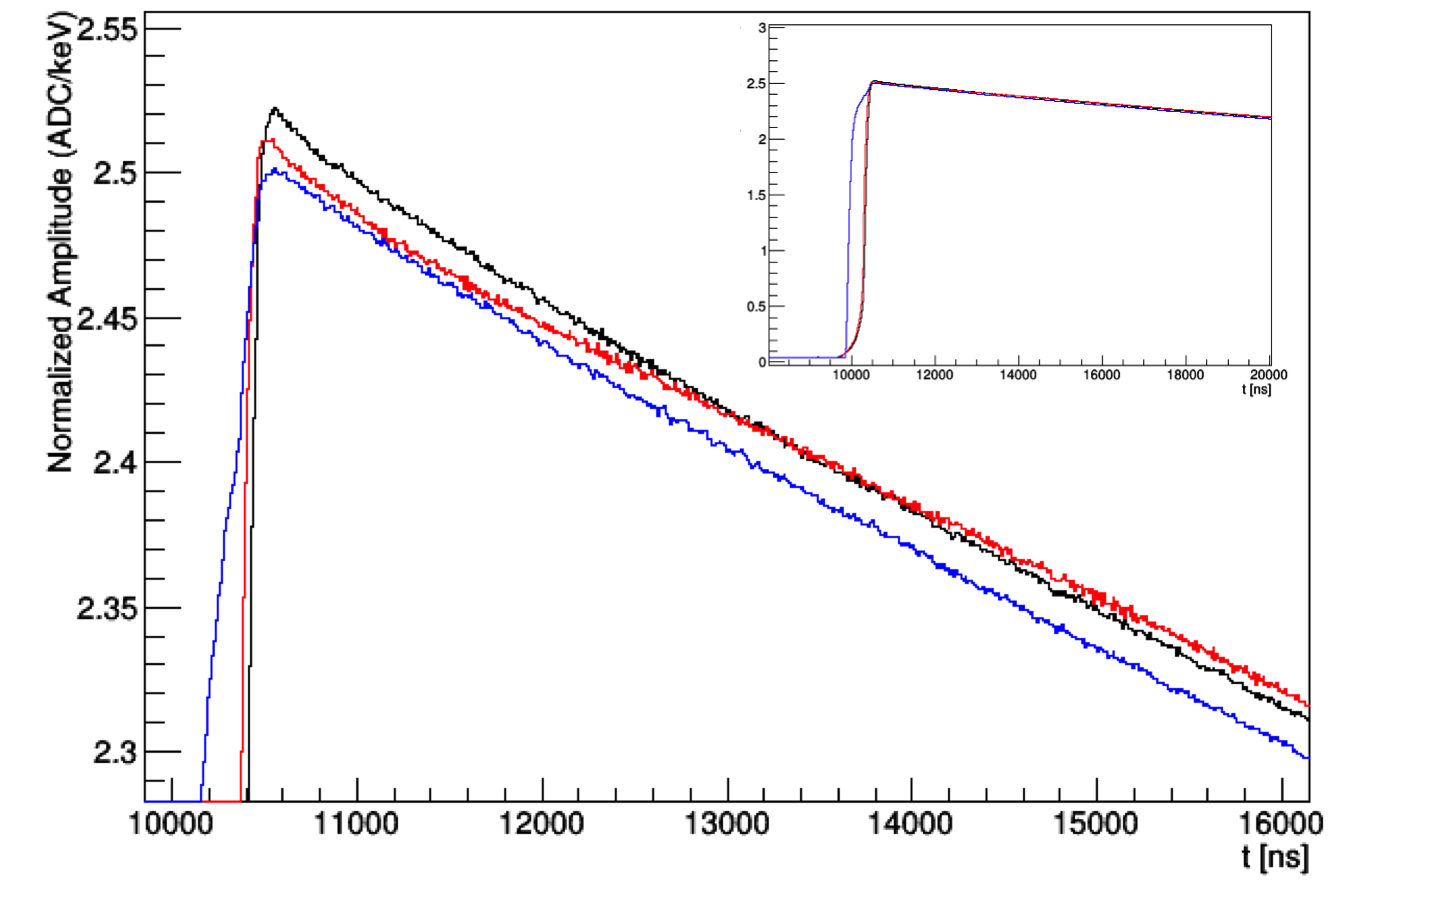
\includegraphics[width=1.0\columnwidth]{/Users/jgruszko/Documents/Thesis/Plots/Ch3/DCR_PS}
 \caption[Sample waveforms demonstrating the effect of pulse-shape on DCR]{The effect of pulse-shape on DCR, in one channel. The event drawn in black passes the DCR cut, those in blue and red fail the cut. The event in blue is thought to be a near-point-contact multi-site event, where the late charge arrival from the second site gives it an ``incorrect" energy for its tail slope. The one in red is thought to be a transition-layer multisite event or an event with high bulk charge trapping, either of which would contribute the additional slow component that changes its tail slope. All events are normalized by their max-pickoff energy ({\tt trapENMCal}), which is the energy estimator used in the DCR calculation.} 
 \label{fig:DCR_PS}
\end{figure}

\subsection{DCR Version 1.1}\label{ssec:dcr_ct}
Version 1.1 of the DCR analysis is currently being tested. This version corrects for the effect of bulk charge trapping in the detectors on the tail slope. It is being developed in an attempt to reduce the pulse-shape systematic uncertainty of the cut acceptance. Correcting for this effect will also reduce the overall width of the DCR distribution, allowing for a more effective cut at the same level of bulk-event sacrifice, and correct the slight broadening of the DCR distribution with increasing energy. 
 
\subsubsection{Bulk Charge Trapping and the DCR Distribution}
The bulk charge trapping in a given detector can be measured by its energy resolution improvement when the effective pole-zero charge trapping correction is applied. Using this method we can comparing the DCR vs. energy distributions for high charge-trapping detectors and low charge-trapping detectors, as in Fig.~\ref{fig:ct_DCRvE}. It is clear that for detectors with minimal charge trapping, the DCR distribution is narrower and that all portions of a peak, like the $^{208}$Tl double escape peak (DEP) shown, have consistent DCR acceptance. For a detector with high charge-trapping, on the other hand, the low-energy tail, which contains the events in which charge-trapping has occurred, has higher DCR values than the bulk of the peak. This matches the effect that would be expected if bulk trapped charge were being released on a 2-3 $\mu$s timescale, adding a slow additional component to the tail slope and making it less negative. 

This effect contributes to $\sigma_{PS}$ because the gaussian portion of the DEP is made up of events that are particularly unlikely to have been affected by bulk charge trapping (since if they were affected by trapping, they would occur in the low-energy tail of the peak). In detectors that have high bulk charge-trapping, this peak will therefore have higher DCR acceptance than the Compton continuum, which is made up of events with a normal incidence of charge trapping, making $\sigma_{PS}$ large for that detector. 

\begin{figure}[]
 \centering
 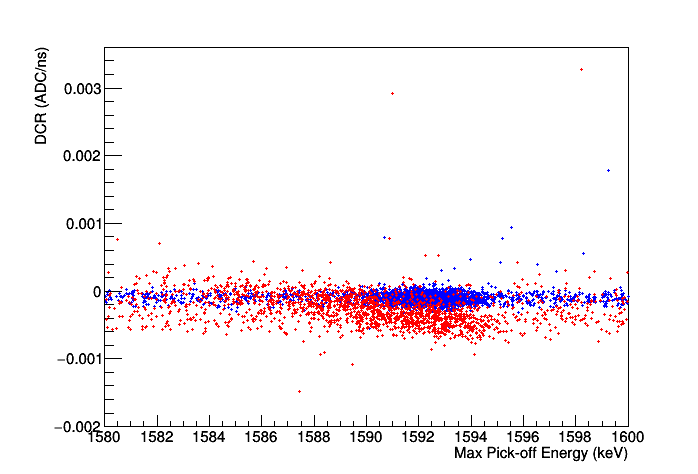
\includegraphics[width=1.0\columnwidth]{/Users/jgruszko/Documents/Thesis/Plots/Ch3/ChargeTrappingStudy_trapENMCal.png}
 \caption[The effect of bulk charge trapping on DCR in the $^{208}$Tl DEP and surrounding continuum.]{The effect of bulk charge trapping on DCR in the $^{208}$Tl DEP and surrounding continuum. The points in red are from detector P42537A, which exhibits a 3 keV FWHM improvement in the 2614 keV peak when charge-trapping is corrected. The points in blue are from detector P42661A, which exhibits a 0.4 keV improvement. The energy shown here, which is used to calculate the DCR value, is {\tt trapENMCal}. This max pick-off energy does not employ the charge-trapping correction.} 
 \label{fig:ct_DCRvE}
\end{figure}

The presence of bulk charge trapping also broadens the overall DCR distribution, increasing the tail of the distribution with high values of DCR. The amount of trapped charge in an event at a given position in the crystal is expected to be a constant fraction of the total energy, so the broadening due to this effect will increase with energy. This causes the fall in DCR cut efficiency with increasing energy observed at higher-sacrifice cuts, as seen in the left-hand plot of Fig.~\ref{fig:singleCh_eff}. 

\begin{figure*}[t]
 \centering
 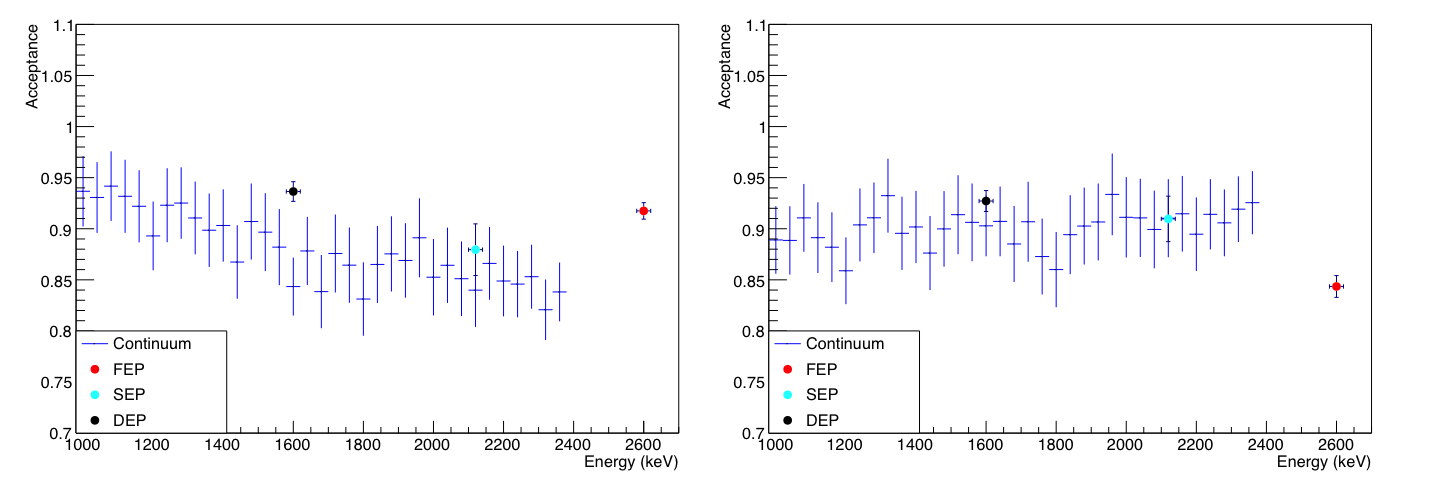
\includegraphics[width=1.0\textwidth]{/Users/jgruszko/Documents/Thesis/Plots/Ch3/sample_eff_dcr90}
 \caption[DCR cut efficiency and uncertainties]{Efficiency plots for the 90\% acceptance DCR cut in P42537A, DS3. {\it Left:} DCR cut efficiency. The pulse-shape systematic uncertainty for the channel can be calculated from the values indicated on this plot, and the energy-scale effect is clearly visible. {\it Right:} The charge-trapping-corrected DCR efficiency. The correction has reduced $\sigma_{PS}$ and the overall energy dependence has been corrected, but the efficiency is lower than expected in the full-energy 2614 keV peak. This requires further study.} 
 \label{fig:singleCh_eff}
\end{figure*}

\subsubsection{Correcting DCR for Charge Trapping}
The charge trapping effect on DCR can be corrected because the distinctive trapping and re-release timescales can be calculated from calibration data. Therefore, for a known level of charge trapping in an event, its re-release effect on the waveform tail can be subtracted from $\delta$, and then the DCR parameter can be calculated in the usual fashion from the remaining tail slope. 

The amount of charge trapping in a given event can be quantified; it is given by the difference between the charge trapping-uncorrected and corrected energies, $\Delta E$:
$$\Delta E =  {\tt trapENFCal}-{\tt trapENMCal} $$
The dependence of $\delta$ on the trapping is found by plotting $\delta$ vs. $\Delta_{E}$ and fitting with a line of slope $\ell_{E}$, as Fig.~\ref{fig:DeltaE}. The energy dependence of this slope is then fit with an exponential function, shown in Fig.~\ref{fig:DeltaEfit}. Then, for a given event, the charge trapping-corrected tail slope $\delta_{CTC}$ is:
$$\delta_{CTC} = \delta - (Ae^{\lambda E})\Delta E$$
where $A$ and $\lambda$ are the parameters found in the exponential fit.The DCR parameters are then calculated as in Version 1.0, leading to a narrower DCR distribution, with less of a high-DCR tail, as in Fig.~\ref{fig:ct_corr_DCR}.

Preliminary tests show that the use of the charge trapping correction improves $\sigma_{PS}$ and the energy-dependence of the DCR cut in detectors with significant charge trapping, but further study is needed to understand its effect in the full-energy peak. See Fig.~\ref{fig:singleCh_eff}. 

\begin{figure}[]
 \begin{subfigure}[t]{.45\textwidth}
 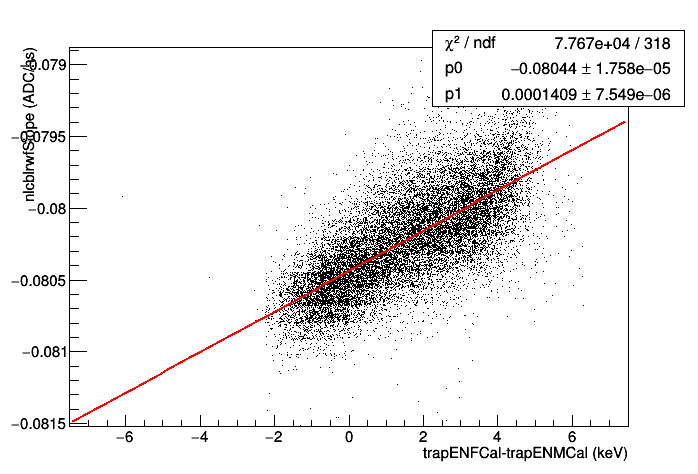
\includegraphics[width=1.0\columnwidth]{/Users/jgruszko/Documents/Thesis/Plots/Ch3/DeltaE}
 \caption{$\delta$ vs. $\Delta$E is plotted and fit with a line of slope $\ell_E$, in red, for each energy peak.}
 \label{fig:DeltaE}
 \end{subfigure}
~
 \begin{subfigure}[t]{.45\textwidth}
 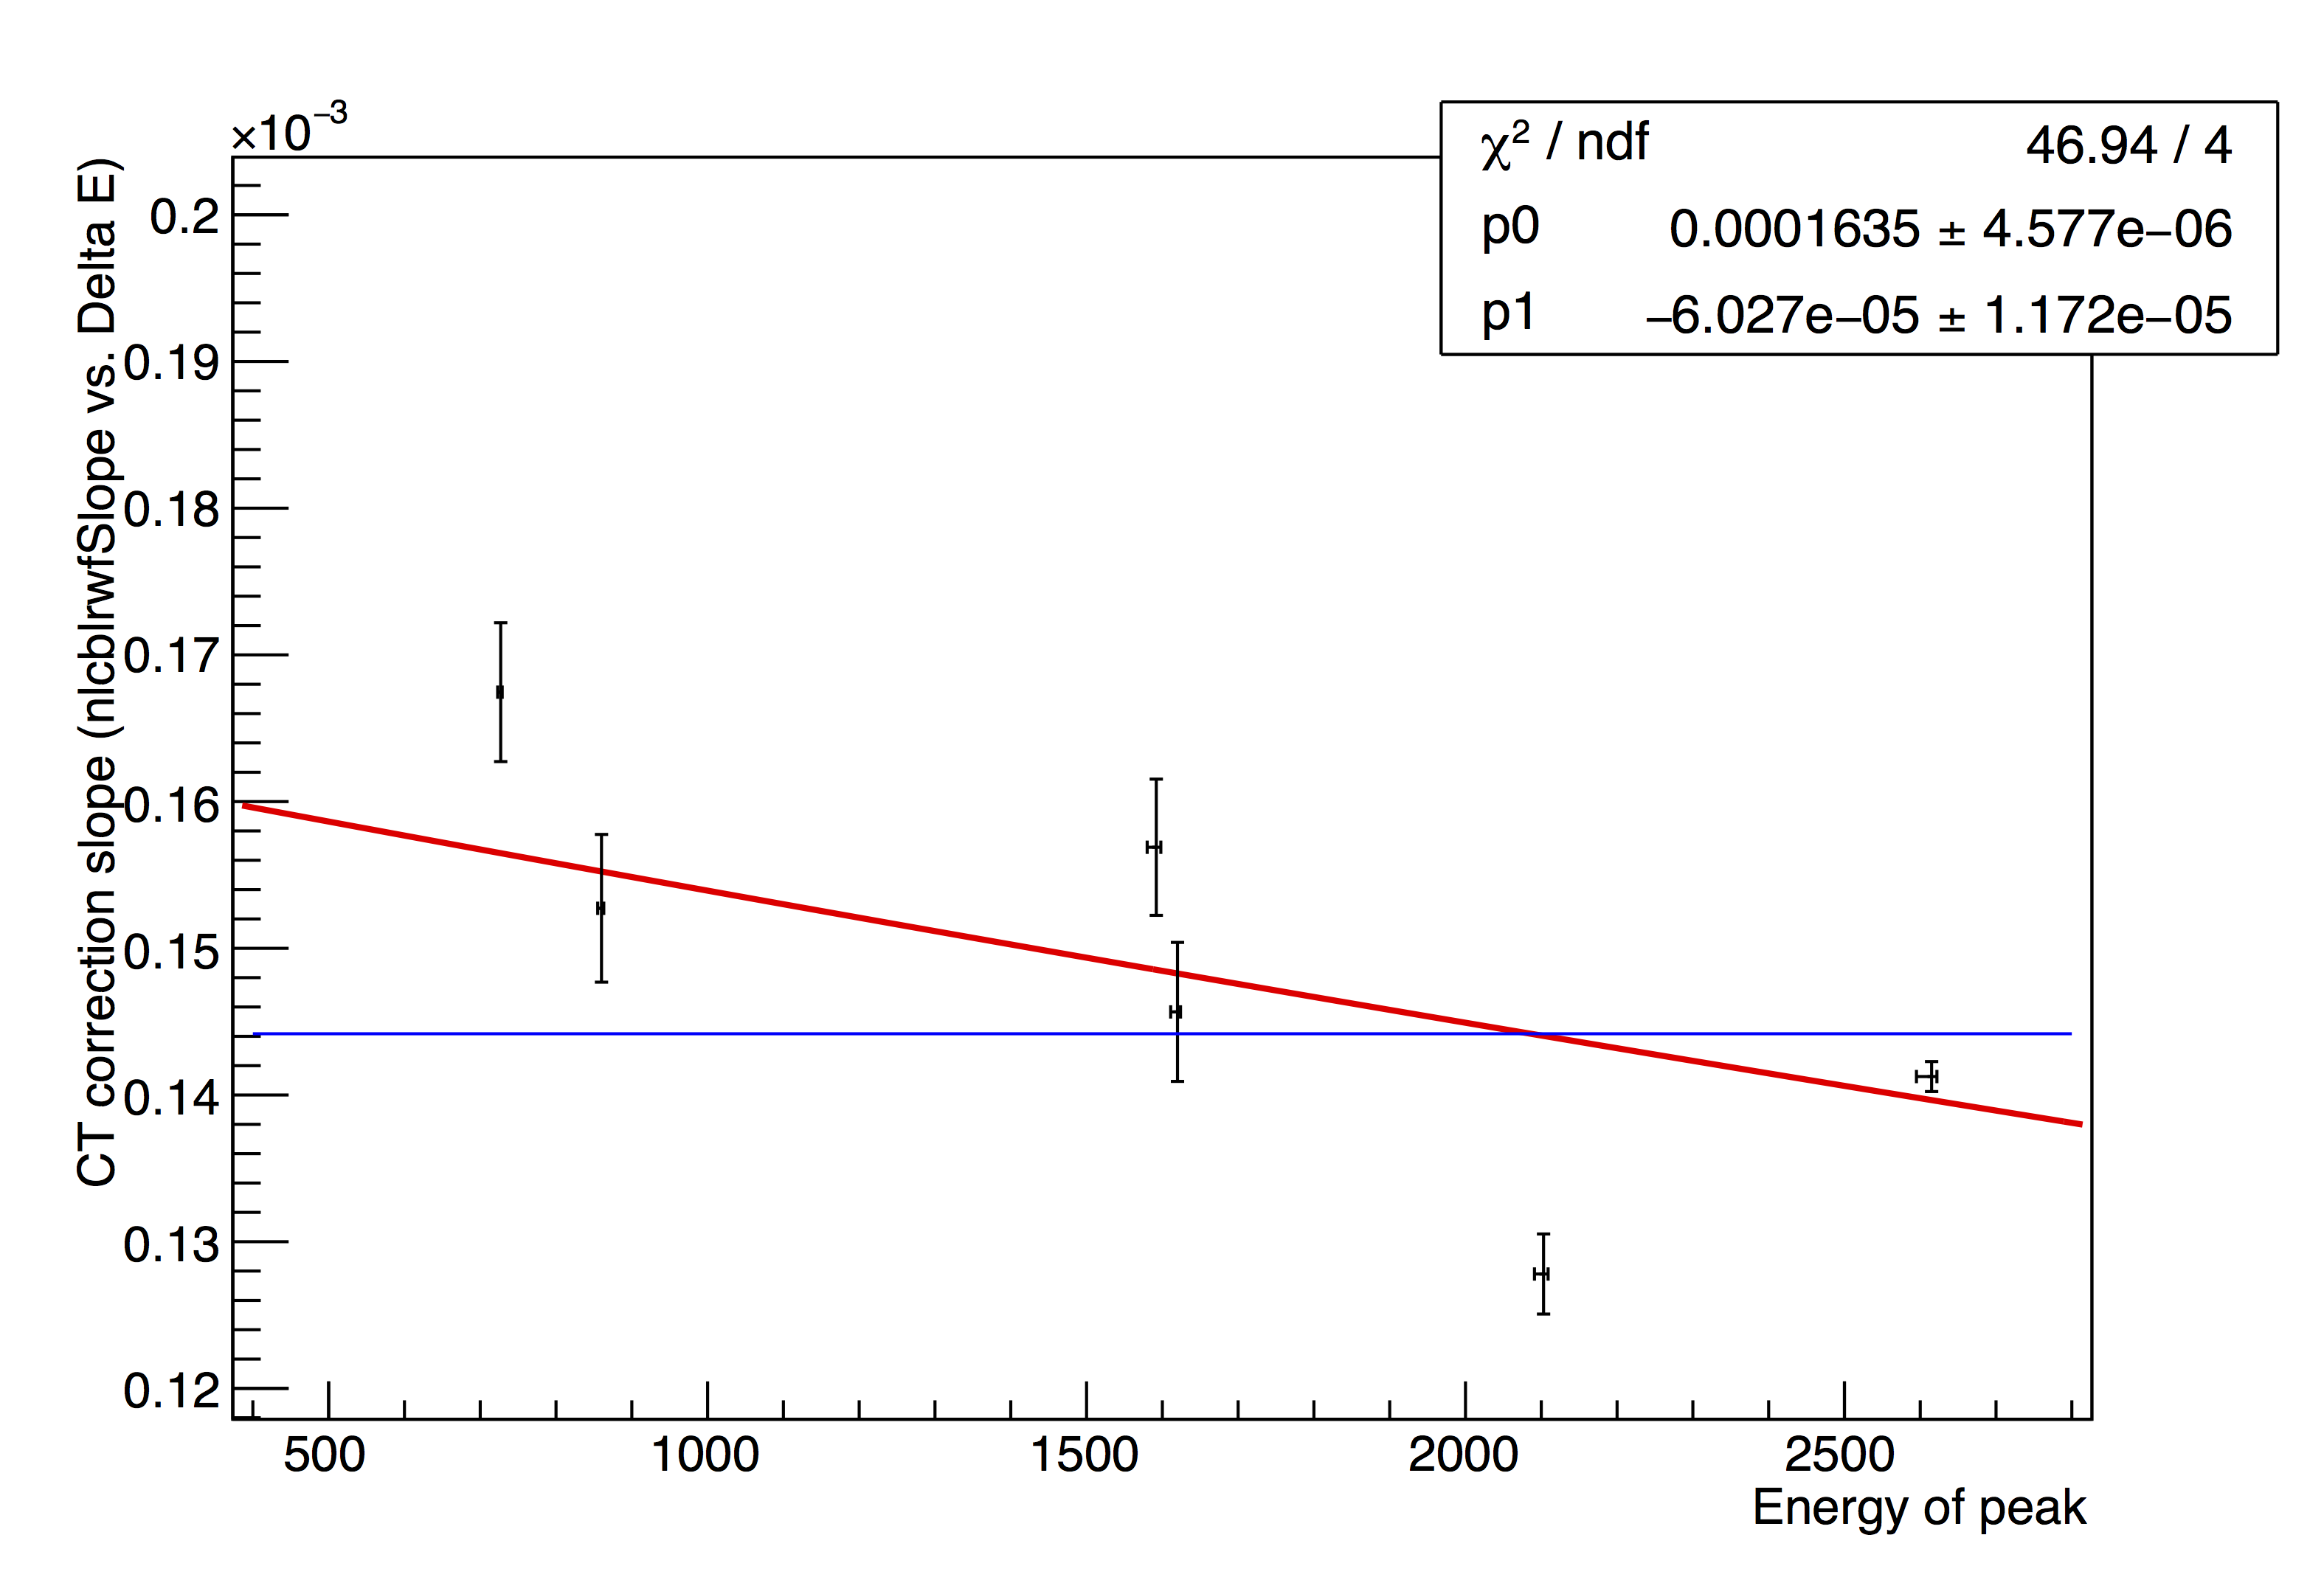
\includegraphics[width=1.0\columnwidth]{/Users/jgruszko/Documents/Thesis/Plots/Ch3/DeltaEfit.png}
 \caption{$\ell_E$ is plotted with respect to E and fit with an exponential, in red. The assumption of constant $\ell_E$, in blue, is a poor model of the observed behavior.}
 \label{fig:DeltaEfit}
 \end{subfigure}
   \centering
 \begin{subfigure}[]{.7\textwidth}
 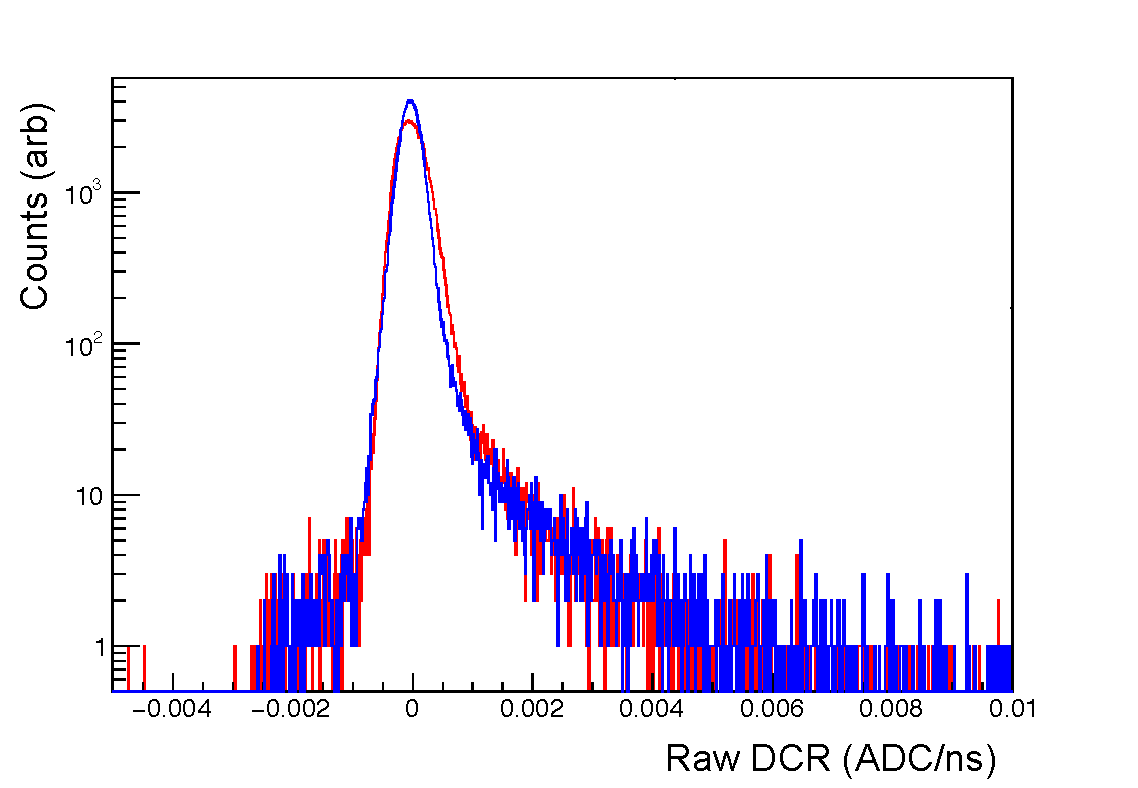
\includegraphics[width=1.0\columnwidth]{/Users/jgruszko/Documents/Thesis/Plots/Ch3/ct_corr_DCR}
 \caption{When corrected using the resulting parameters, the charge-trapping-corrected DCR distribution in the 1 to 2.38\,MeV range, in blue, is narrower and with a smaller high-DCR tail than the uncorrected distribution, in red.}
 \label{fig:ct_corr_DCR}
 \end{subfigure}
 \caption[The steps of the charge trapping tail slope correction]{The steps of the charge trapping tail slope correction, in P42537A, a high charge trapping detector in DS3.} 
 \label{fig:ct_corr}
\end{figure}

These tests have also shown that the calibration of {\tt trapENM} is not reliable enough to use as an indicator of the amount of trapped charge in every detector. Depending on how the calibration of the energy is conducted, the peak positions may be offset by up to several keV in some channels, leading to unphysical negative amounts of trapped charge. 

Though version 1.1 of the analysis is a good proof-of-concept, demonstrating that charge trapping is leading to significant broadening of the DCR distribution and to the large observed pulse-shape uncertainty, it is not the best path forward to reliably correcting for this effect. 

\subsection{DCR Version 2.0}
\subsubsection{True Pole-Zero Correction}
Future versions of the DCR analysis could be improved by applying de-convolving the full electronic response function for the channel from the pulse before searching for a remaining slow component. This component could be identified either using a two-point slope estimator, like the one used in version 1, or some other method. One possible approach is to use a passivated-surface-collection waveform template, and apply the goodness-of-fit as the DCR discriminator. 

Preliminary work on the TUBE scanning system, using a two-point slope estimator after pole-zero correction, shows that this approach gives a narrower distribution for bulk events, particularly for energies over 3 MeV, where muons and multisite events dominate. This approach leads to improved discrimination of passivated surface events in this system, which has a high background rates. See Fig.~\ref{fig:dcr_dcrpzc_comparison}.

If a true pole-zero correction were employed in the DCR algorithm, the stability uncertainty of the DCR parameters could be reduced by re-tuning the decay constant for each detector with each weekly energy calibration of the \DEM. In the effective correction used in version 1 of the analysis, multi-hour calibration runs are needed to re-tune the parameters; therefore, physics live time considerations prevent regular re-tuning. A true pole-zero correction, on the other hand, can be determined using very few (less than 500) events, allowing it to be re-tuned using the already-established weekly energy calibrations. 

\subsubsection{Charge Trapping Correction}
Further work is also being done on a waveform-by-waveform charge-trapping correction, which uses the drift time of the pulse to calculate the expected amount of charge lost in the bulk. Early results indicate that this approach is more reliable than the estimate of $\Delta E$ used in version 1.1, and dramatically reduces the width of the DCR distribution, allowing for more effective surface event discrimination. 

%
%\begin{figure*}[]
 %\centering
 %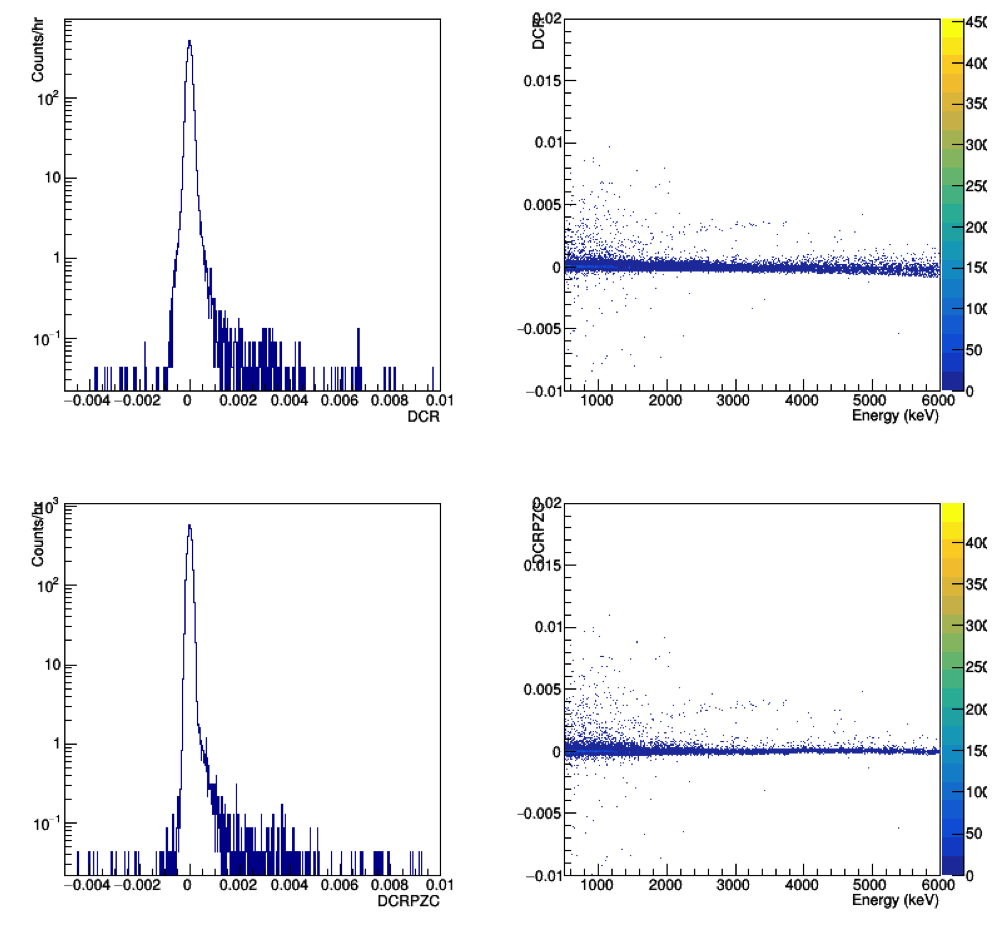
\includegraphics[width=.8\textwidth]{/Users/jgruszko/Documents/Thesis/Plots/Ch3/TUBE_DCRPZ}
 %\caption[A comparison of v1.0 and v2.0 of the DCR analysis, in the TUBE system]{Preliminary tests of version 2.0 of the DCR parameter, in the TUBE scanning system. {\it Top:} The version 1.0 DCR distributions, for energies between 1 and 6~MeV. {\it Bottom:} The version 2.0 DCR distributions. The two-point slope DCR parameter is calculated and applied after a pole-zero correction is used to de-convolve the electronics response function. The use of version 2 leads to a narrower bulk-event distribution, particularly at energies above 3 MeV, where muons and multisite events dominate.} 
% \label{fig:TUBE_v2}
%\end{figure*}

%%%%%% This is a results section %%%%%%
\section{\MJ\ Analysis}
\subsection{Efficiencies}
In each channel, the average acceptance for single-site events (after data-cleaning) in the Compton continuum region, taken to be from 1\,MeV to 2.38\,MeV, is set to match the quoted acceptance of the cut. For instance, {\tt dcr99} has average bulk acceptance of 99\%, as nearly as is allowed by the finite statistics of the sample used to set the cut. 

The true acceptance for the \nonubb\ region is calculated from that energy region directly, also using calibration data, due to the energy non-linearity effect, as discussed above. It is given in Table~\ref{tab:DS_efficiencies} for each of the data sets.  

\subsection{Uncertainties}

\begin{table}[]
\centering
\begin{tabular}{l l l l l l l}
Data Set & $\epsilon_{ROI}$ (\%) & $\sigma_{PS}$ (\%) & $\sigma_{stab}$  (\%) & $\sigma_{stat}$  (\%) &$\sigma_{tot}$ (\%) \\ 
\hline
DS0  & 98.1  &  0.8  &    &  0.1  &  0.9 \\   
DS1  & 95.6  &  1.1  &    &  0.1  &  1.1 \\
DS2  & 98.6  &  0.9  &    &  0.2  &  1.0 \\
DS3  & 99.1  &  0.9  &    &  0.1  &  0.9 \\
DS4  & 98.9  &  1.2  &    &  0.1  &  1.2 \\
DS5a  & 92.1  &  0.7  &    &  0.3  &  0.8 \\
DS5b  & 95.8  &  1.4  &    &  0.2  &  1.4 \\
\end{tabular}
 \caption[\nonubb\ efficiency and uncertainties in the \MJ\ \DEM]{\nonubb\ efficiency and uncertainties, given for high gain channels in each data set. DS5 was split into DS5a and DS5b because the presence of elevated electronic noise in DS5a (due to known ground loop problems) drastically reduced the effectiveness of the DCR cut in these runs.} 
 \label{tab:DS_efficiencies}
\end{table}

As discussed, the pulse shape systematic uncertainty and uncertainty due to cut instability dominate, with the statistical uncertainties contributing about 0.2\% and the energy scale uncertainty contributing negligibly. The uncertainties for each data set are given in Table~\ref{tab:DS_efficiencies}. 

\subsection{DCR Validation in Low-Background Data}

\begin{figure*}[]
 \centering
 \begin{subfigure}[t]{0.45\textwidth}
   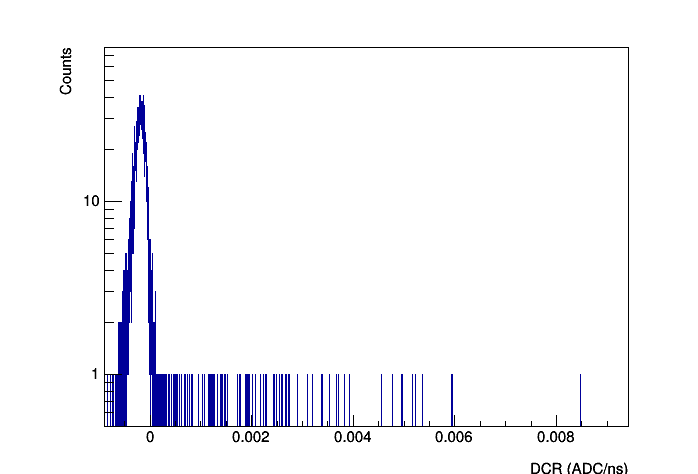
\includegraphics[width=\textwidth]{/Users/jgruszko/Documents/Thesis/Plots/Ch3/DS3_DCR_HG}
    \caption{The DCR distribution.}
    \label{fig:DS3_DCR}
  \end{subfigure}
\hfill
 \begin{subfigure}[t]{0.45\textwidth}
   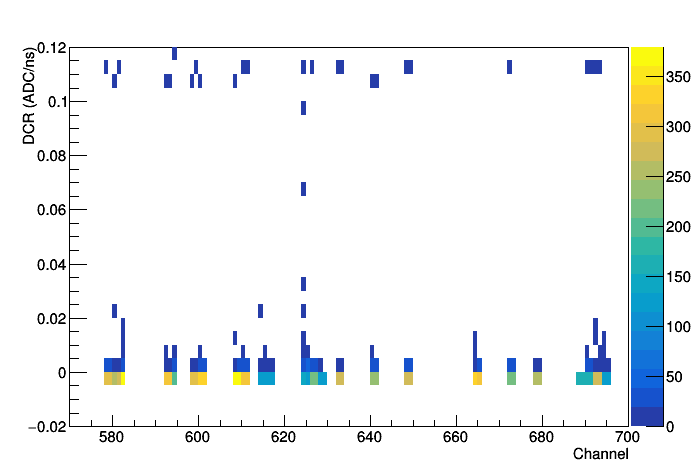
\includegraphics[width=\textwidth]{/Users/jgruszko/Documents/Thesis/Plots/Ch3/DS3_DCRvCh}
    \caption{The DCR distribution for each channel.}
    \label{fig:DS3_DCRvCh}
  \end{subfigure}
   ~
 \begin{subfigure}[t]{0.45\textwidth}
   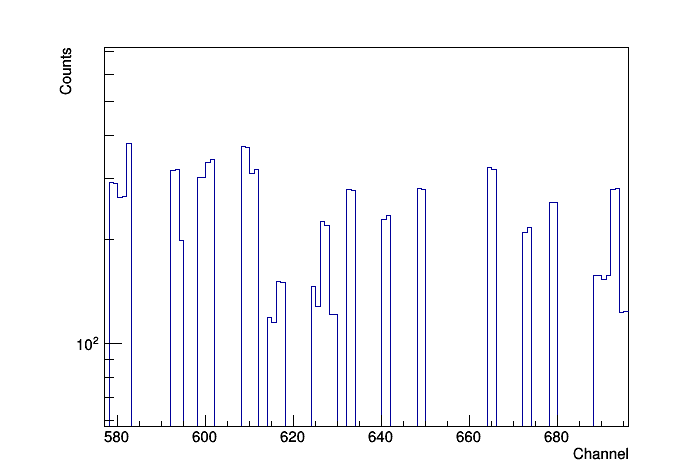
\includegraphics[width=\textwidth]{/Users/jgruszko/Documents/Thesis/Plots/Ch3/DS3_events_byCh}
    \caption{The number of events remaining after the DCR cut, in each channel.}
    \label{fig:events_byCh}
  \end{subfigure}
\hfill
  \begin{subfigure}[t]{0.45\textwidth}
   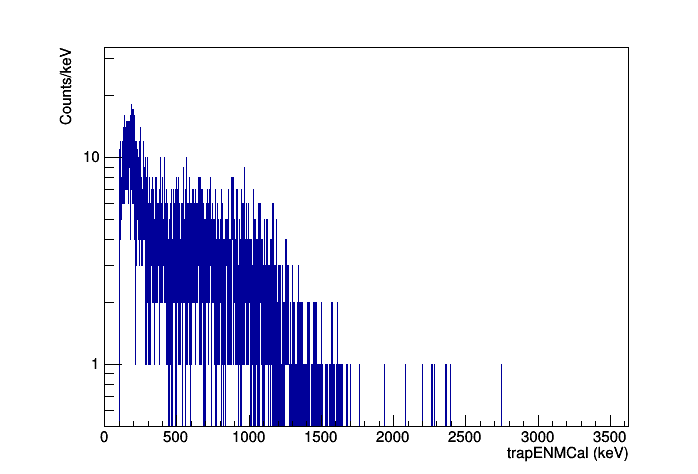
\includegraphics[width=\textwidth]{/Users/jgruszko/Documents/Thesis/Plots/Ch3/DS3_E_HG}
    \caption{The spectrum after the DCR cut is applied.}
    \label{fig:DS3_E_HG}
  \end{subfigure}
   ~
  \begin{subfigure}[t]{0.45\textwidth}
   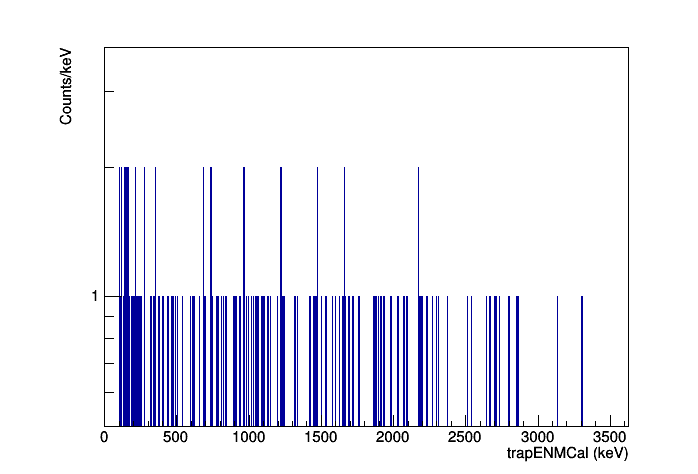
\includegraphics[width=\textwidth]{/Users/jgruszko/Documents/Thesis/Plots/Ch3/DS3_Ecut_HG}
    \caption{The spectrum of events cut by DCR.}
    \label{fig:DS3_Ecut_HG}
  \end{subfigure}
\hfill
     \begin{subfigure}[t]{0.45\textwidth}
   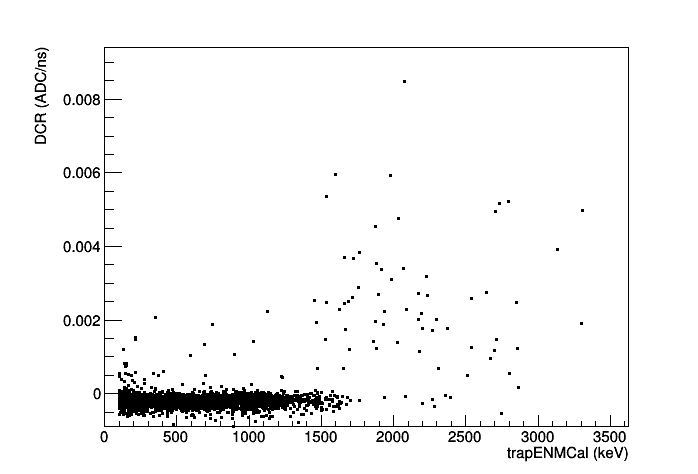
\includegraphics[width=\textwidth]{/Users/jgruszko/Documents/Thesis/Plots/Ch3/DS3_DCRvE_HG}
    \caption{The DCR vs. energy distribution.}
    \label{fig:DS3_DCRvE_HG}
  \end{subfigure}
  \caption{The results of DCR validation for DS 3 high gain channels.}
  \end{figure*}
  
 \begin{figure}[t]
   \centering
   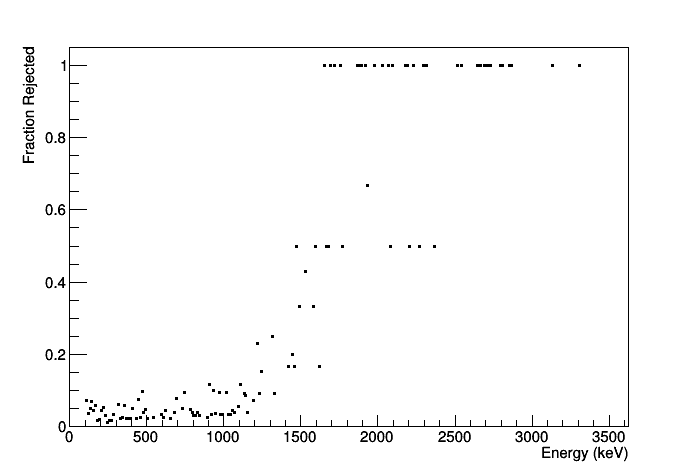
\includegraphics[height=3in]{/Users/jgruszko/Documents/Thesis/Plots/Ch3/DS3_DCRrej}
    \caption{The DCR rejection fraction as a function of energy, in DS 3 high gain channels.}
    \label{fig:DS3_DCRrej}
  \end{figure}

The DCR in each background skim data set is checked using a dedicated validation script, which is used to check for channels in which the DCR parameters are not being applied correctly, unexpected energy dependence, and other errors in the DCR parameters.  The validation script is applied first to the open data, and then, after unblinding, to the remaining data. This script produces the following plots:
\begin{itemize}
\item The DCR distribution in the channel: It should have an roughly gaussian shape, with a high-DCR tail extending to the right. The peak should be centered at a DCR value less than 0. See Fig.~\ref{fig:DS3_DCR}. If a channel does not have a DCR cut available, a sharp (single-bin-width) spike will appear at 0 along with the gaussian for the correctly calculated parameters. 
\item The DCR distribution for each channel: Each distribution should be peaked just below 0, with a tail extending to high-DCR values. All events appearing at 0, or a peak appearing in a different location, are indications of errors in the DCR parameters. See Fig.~\ref{fig:DS3_DCRvCh}.
\item The number of events retained by the DCR cut in each channel: All bins should be similar in height. See Fig.~\ref{fig:events_byCh}.
\item The energy spectrum after the DCR cut is applied: It should resemble the \twonubb spectrum at energies above 500\,keV, with no large dips at any particular energies. There should be few events remaining above 1.8\,MeV. See Fig.~\ref{fig:DS3_E_HG}.
\item The energy spectrum of the events removed by the DCR cut: It should be roughly flat, with a small rise at low energy. See Fig.~\ref{fig:DS3_Ecut_HG}.
\item The DCR vs. energy distribution of events: Most events above 1.8\,MeV should have visibly high DCR. Below 1.5\,MeV, most events should have DCR below 0. See Fig.~\ref{fig:DS3_DCRvE_HG}.
\item The DCR rejection efficiency as a function of energy, in 10\,keV bins: It should be at or near 1 in most bins above 1.8\,MeV, and fall to approximately 10\% (i.e. the set cut bulk-acceptance) at energies below 1\,MeV. See Fig.~\ref{fig:DS3_DCRrej}.
\end{itemize}

If no anomalies or major instabilities (see above) are found, the DCR cut is ready to be used in spectral analysis. 

